\documentclass[10pt]{article}
\usepackage{icmlko}

\icmlmeta{IP 파운데이션 월드모델}{129}{의심은 근거가 아니다}{웹툰을 같은 플랫폼이라고 미리 뺐는데, 재 보니 뺄 이유가 없었다 --- 그리고 내 팝업 가설도 스스로 무너졌다}

\begin{document}

\twocolumn[
\icmlheader

\begin{abstract}
노트 128에서 웹툰만 빼고 검색 축을 붙였다. 이유는 그럴듯했다 --- 웹툰
라벨은 네이버 웹툰 즐겨찾기이고 축은 네이버 검색이니 \emph{같은 플랫폼}이고,
노트 119--121이 잰 결합(자기 $\rho$의 21$\sim$38\%가 부풀림)이 걸릴 수
있다. \textbf{그런데 그건 의심이지 근거가 아니었다.} 이번에 긁어서 쟀다.
웹툰의 검색--라벨 상관은 $+$0.327로 결합 없는 도메인 여섯의 분포
($+$0.209 $\pm$ 0.143) 안에 있고 게임($+$0.402)보다 낮다. 더 결정적인 것은
\textbf{덮음을 맞춘 비교}다 --- 모바일(덮음 41.3\%)의 이득이 $+$0.099인데
웹툰(37.9\%)은 $+$0.063으로 \emph{오히려 낮다}. 결합이 있었다면 웹툰이
튀어야 하는데 안 튄다. 그래서 넣었다. \textbf{판 $\rho$가 다시 올랐다} ---
부스팅이 $+$0.4019에서 \textbf{$+$0.4107}, 귀무 대비 $z$가 $+$5.39에서
\textbf{$+$6.57}, 귀무 폭이 0.0752에서 \textbf{0.0630}으로 좁아졌다. 공통
다섯 축만 쓰던 $+$0.3363에서 총 \textbf{$+$0.0744}다. \textbf{그리고 내
가설이 하나 무너졌다.} 노트 128에서 ``팝업만 내리는 것은 검색이 규모
신호인데 팝업 라벨이 규모를 나눠 버린 일평균이기 때문''이라 적었고, 실제로
원상관이 총량 $+$0.220 대 일평균 $+$0.088로 갈렸다. 그래서 팝업 라벨을
총량으로 바꿔 하네스에 넣었다. \textbf{여전히 음수였다}($-$0.039 대
$-$0.058). $n$=67에서 $+$0.220과 $+$0.088의 차이는 표준오차 0.12 안이었고,
하네스가 그것을 확인해 줬다. 팝업은 그냥 브랜드 사전 검색으로 안 풀린다.
\end{abstract}
]

\begin{figure*}[t]
\centering
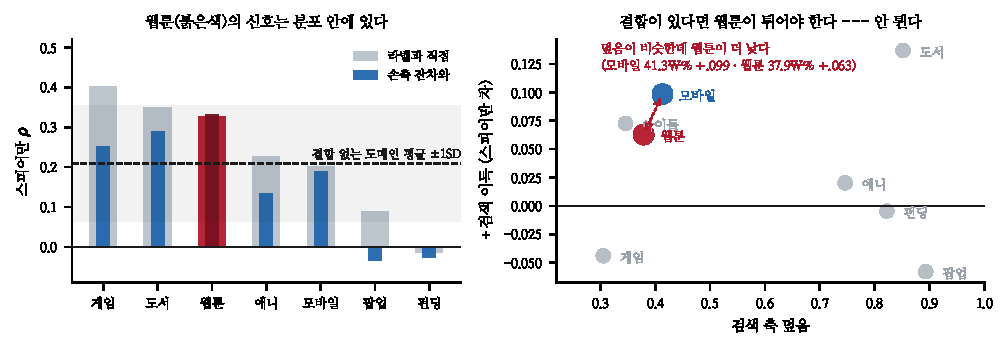
\includegraphics[width=\textwidth]{figs/couple.pdf}
\caption{왼쪽 --- 웹툰(붉은색)의 신호는 결합 없는 도메인의 분포 안에 있다.
오른쪽 --- 결합이 있다면 웹툰이 위로 튀어야 하는데, 덮음이 비슷한 모바일보다
오히려 낮다.}
\end{figure*}

\section{빼 놓고 재지 않은 것}

노트 128은 도메인 여덟에 검색 축을 붙이면서 웹툰만 뺐다. 근거로 적은 것은
노트 117의 출처 차단 --- 라벨을 만든 플랫폼의 다른 계수기에서 나온 축은
상관이 낮아도 안 쓴다는 규칙이다. 웹툰 라벨(네이버 즐겨찾기)과 축(네이버
검색)은 그 조건에 맞는다.

문제는 그 규칙을 \emph{적용만 하고 검정하지 않았다}는 것이다. 웹툰은 후행
표본 711건으로 제일 큰 대상이다. 제일 큰 것을 의심만으로 빼면 안 된다.

\claimx{\textbf{결합은 막을 이유가 아니라 잴 대상이다.} 긁어 놓고 결합이
없는 도메인들의 분포와 견주면 된다. 결합이 실재하면 웹툰의 신호가 그
분포 위로 튀어야 한다.}{``튀면 결합''은 필요조건이지 충분조건이 아니다.
웹툰이 원래 예측하기 쉬운 도메인일 수도 있다 --- 아래 덮음 맞춘 비교가
그 걱정을 일부 덜어 준다.}

1{,}064건을 긁어 덮음 37.9\%를 얻었다(할당량 소진으로 중단).

\section{웹툰은 안 튄다}

\begin{table}[t]
\centering\tsize
\caption{검색 축(수준)과 라벨의 상관, 그리고 손으로 매긴 축 다섯으로 맞춘
잔차와의 상관. $\bigstar$ 는 라벨과 축이 같은 플랫폼.}
\begin{tabular}{lrrrl}
\toprule
& 덮음 & 라벨과 & 잔차와 & 라벨 출처 \\
\midrule
게임 & 30.5\% & $+$.402 & $+$.253 & 스팀 \\
도서 & 85.2\% & $+$.350 & $+$.289 & 알라딘 \\
\textbf{웹툰}$\bigstar$ & 37.9\% & $+$.327 & $+$.332 & 네이버 즐겨찾기 \\
애니 & 74.6\% & $+$.226 & $+$.133 & 라프텔 \\
모바일 & 41.3\% & $+$.200 & $+$.188 & 앱스토어 \\
팝업 & 89.3\% & $+$.088 & $-$.034 & 현장 방문자 \\
펀딩 & 82.2\% & $-$.014 & $-$.027 & 텀블벅 \\
\bottomrule
\end{tabular}
\end{table}

\claimx{\textbf{웹툰의 라벨 상관은 분포 안이다.} 결합 없는 여섯의 평균이
$+$0.209, 표준편차 0.143이고 웹툰은 $+$0.327 --- $+$0.83 표준편차다. 게임이
$+$0.402로 더 높다.}{잔차 상관에서는 웹툰이 $+$0.332로 제일 높다($+$1.55
표준편차). 비교 대상이 여섯뿐이라 이 정도 위치는 결정적이지 않다.}

잔차 쪽이 조금 걸려서 더 직접적인 검정을 했다. 결합이 있다면 그것은
\emph{이득}으로 나타나야 한다 --- 그리고 이득은 덮음에 크게 끌리므로
덮음이 비슷한 도메인끼리 견줘야 한다.

\claimx{\textbf{덮음이 거의 같은데 웹툰의 이득이 더 작다.} 모바일 덮음
41.3\%에 이득 $+$0.099, 웹툰 덮음 37.9\%에 이득 $+$0.063이다. 결합이
있었다면 반대 방향이어야 한다.}{한 쌍의 비교다. 그리고 두 도메인은 라벨
정의도 다르다(앱스토어 평점 수 대 즐겨찾기 수).}

\section{그래서 넣었고, 최고치가 갱신됐다}

\begin{table}[t]
\centering\tsize
\caption{판 $\rho$ · 배포 규약 $T$=2025.0 · 가드 일곱 전부 통과.
$+$검색은 웹툰까지 포함한 판.}
\begin{tabular}{lrrrr}
\toprule
& 공통 다섯 & $+$검색 & 귀무 폭 & $z$ \\
\midrule
F8 부스팅 & $+$.3363 & \textbf{$+$.4107} & .0630 & \textbf{$+$6.57} \\
F9 짝 순위 & $+$.3464 & $+$.3891 & .1041 & $+$3.89 \\
F10 도메인별 수축 & $+$.3452 & $+$.3872 & .0926 & $+$4.27 \\
F6 직접 풀링 & $+$.3413 & $+$.3843 & .0966 & $+$4.12 \\
\bottomrule
\end{tabular}
\end{table}

\claimx{\textbf{웹툰을 넣어 얻은 것이 $+$0.009$\sim$$+$0.016이다.} 부스팅
$+$0.4019 $\to$ $+$0.4107, 짝 순위 $+$0.3736 $\to$ $+$0.3891, 직접 풀링
$+$0.3704 $\to$ $+$0.3843. 의심만으로 뺐다면 이만큼을 버릴 뻔했다.}{웹툰
덮음이 37.9\%에서 멈춰 있다(할당량). 나머지를 채우면 더 갈 여지가 있다.}

\begin{figure*}[t]
\centering
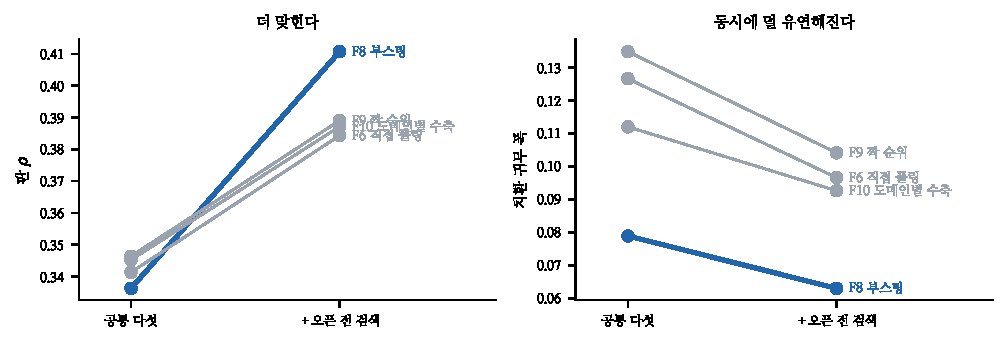
\includegraphics[width=\textwidth]{figs/climb.pdf}
\caption{왼쪽 --- 더 맞힌다. 오른쪽 --- 동시에 덜 유연해진다. 노트 126의
법칙이 경계하던 방향의 반대다.}
\end{figure*}

\claimx{\textbf{귀무 폭이 계속 좁아진다.} 부스팅이 0.0789에서 0.0630으로,
직접 풀링이 0.1266에서 0.0966으로 줄었다. 축이 늘면 보통 유연해지는데
여기서는 반대다 --- 전 도메인이 공유하는 축이라 우연히 잘 보일 길이
오히려 줄어든다.}{귀무는 치환 99회로 잰 것이라 폭 자체에 오차가 있다.
0.0752 대 0.0630 같은 차이는 그 오차 안일 수 있다.}

\section{그리고 내 가설이 무너졌다}

노트 128에서 팝업만 내리는 것을 이렇게 설명했다 --- 검색은 \emph{규모}
신호인데 팝업 라벨은 규모를 나눠 버린 \emph{일평균}이다. 그리고 실제로
원상관이 갈렸다.

\begin{table}[t]
\centering\tsize
\caption{팝업 검색 수준과 세 가지 라벨. $n$=67.}
\begin{tabular}{lr}
\toprule
& $\rho$ \\
\midrule
총량 (y\_total) & $+$0.220 \\
기간 (일) & $+$0.213 \\
일평균 (y\_perday, 현행) & $+$0.088 \\
\bottomrule
\end{tabular}
\end{table}

그럴듯해서 바로 검정했다. 팝업 라벨을 총량으로 갈아 끼우고 하네스에 넣었다.

\claimx{\textbf{틀렸다.} 총량으로 바꿔도 검색 축은 여전히 손해다 ---
$-$0.039(총량) 대 $-$0.058(일평균). 방향은 맞는데 부호를 못 뒤집는다.
$n$=67에서 $+$0.220과 $+$0.088의 차이는 표준오차 0.12 안이었고, 그
차이를 신호로 읽은 것이 성급했다.}{``검색이 규모 신호''라는 것 자체는
다른 도메인에서 여전히 성립할 수 있다. 무너진 것은 ``그래서 팝업이
내린다''는 설명이다.}

남는 것은 더 단순한 사실이다. \textbf{브랜드 사전 검색은 팝업 유입을
예측하지 못한다.} 잔차 상관 $-$0.034가 그 말을 하고, 라벨을 바꿔도 그대로다.

\section{남은 것}

\begin{table}[t]
\centering\tsize
\caption{다음.}
\begin{tabular}{ll}
\toprule
웹툰 & 덮음 37.9\% $\to$ 나머지 (할당량 회복 후) \\
만화 · 세계애니 & 덮음 0\% --- 한국어 제목 매핑이 필요 \\
팝업 & 브랜드 검색은 아니다. 다른 사전 신호를 찾는다 \\
\bottomrule
\end{tabular}
\end{table}

이번 노트의 교훈은 수치가 아니라 절차 쪽이다. 노트 117의 출처 차단은
좋은 규칙인데, \textbf{규칙을 적용하는 것과 규칙이 이 판에서 실제로
걸리는지 재는 것은 다른 일이다.} 제일 큰 대상 하나를 의심만으로 빼고
있었다.

\end{document}
